%%
%% using aastex version 6.3
%% Setup

\documentclass[twocolumn]{aastex631}

\newcommand{\vdag}{(v)^\dagger}
\newcommand\aastex{AAS\TeX}
\newcommand\latex{La\TeX}
\usepackage{amsmath}

\begin{document}

\title{The Morphology of the Stellar Remnant of the Milky Way + M31 Major Merger}

%% Author

\author{Hanga Andras-Letanovszky}
\affiliation{Department of Astronomy, University of Arizona,  933 N Cherry Ave, Tucson, AZ}

%% Submission date
\date{08 May 2025}

% abstract
\begin{abstract}

Morphology, or shape, is a particularly useful way of characterizing the remnants of dry major mergers of spiral galaxies, i.e. collisions between gas-poor spiral galaxies of approximately the same mass.
Studying remnant morphology allows us to identify merger remnants and thus constrain merger rates and their importance in the formation of galaxies, especially elliptical galaxies.
To further investigate this topic, I used the collisionless $N$-body simulation of the Milky Way-M31 merger by \cite{van_der_Marel+2012}, where initial conditions of the two galaxies were set as close as possible to their present states and their particles were then allowed to interact via Newton's law of gravity.
In particular, I studied the three-dimensional morphology of the remnant as a function of radius. 
I found that the structure of the remnant is triaxial throughout, but closer to oblate overall.
This indicates that dry major mergers are more likely to form oblate, or close to oblate, remnants than originally thought; thus, such mergers could be a more significant formation mechanism for a broader range of elliptical galaxies than expected.


\end{abstract}

%% Keywords
% must bold and define at first use in text!
\keywords{Major Merger -- Dry Merger -- Oblate/Prolate/Triaxial -- Spiral Galaxy -- Elliptical Galaxy}

%% Introduction

\section{Introduction}

% Define your proposed topic and how it relates to galaxy evolution
Mergers are collisions of two or more galaxies in which the central nuclei of the galaxies have merged, making it impossible to define multiple distinct centers of mass corresponding to the parent galaxies.
Mergers are classified using multiple factors.
One is the mass ratio of the progenitors: \textbf{major mergers} are mergers of galaxies with roughly equal masses (in the case of binary mergers, a mass ratio of over 1:4), whereas minor mergers have progenitors with a larger mass difference.
% BE MORE SPECIFIC WITH THE RATIO DUMBASS
Another is gas-richness of the merger: wet mergers occur between gas-\textit{rich} galaxies, and \textbf{dry mergers} between gas-\textit{poor} galaxies.
Regardless of the type, though, mergers leave behind a remnant consisting of the stars and gas from the parent galaxies that remained gravitationally bound post-merger. 
% An example of a remnant from a simulated merger is shown in Figure \ref{fig:merger} at $t$ = 2.66 Gyr.
The morphology of the remnant is heavily influenced by the properties of the parent galaxies as well as how the collision occurred \citep{Barnes+1992}, and is descrbed by whether it's more disk-like or elliptical, and whether it contains any substructure; remnants are often \textbf{elliptical galaxies}, which rarely have a disk and contain little to no substructure, as opposed to \textbf{spiral galaxies}, which are disk-like with spiral arms.
% In principle, the 3D structure of the remnant can be described as \textbf{oblate} ("squashed", like a grapefruit), \textbf{prolate} ("stretched", like a football), or \textbf{triaxial} (with all axes different lengths).
% Inherently collisional structures such as tidal arms and bridges are also often observed, and these in particular frequently help identify galaxies formed in mergers \citep{Duc2013}.
% \begin{figure}[h!]
%     \centering
%     \centering
%     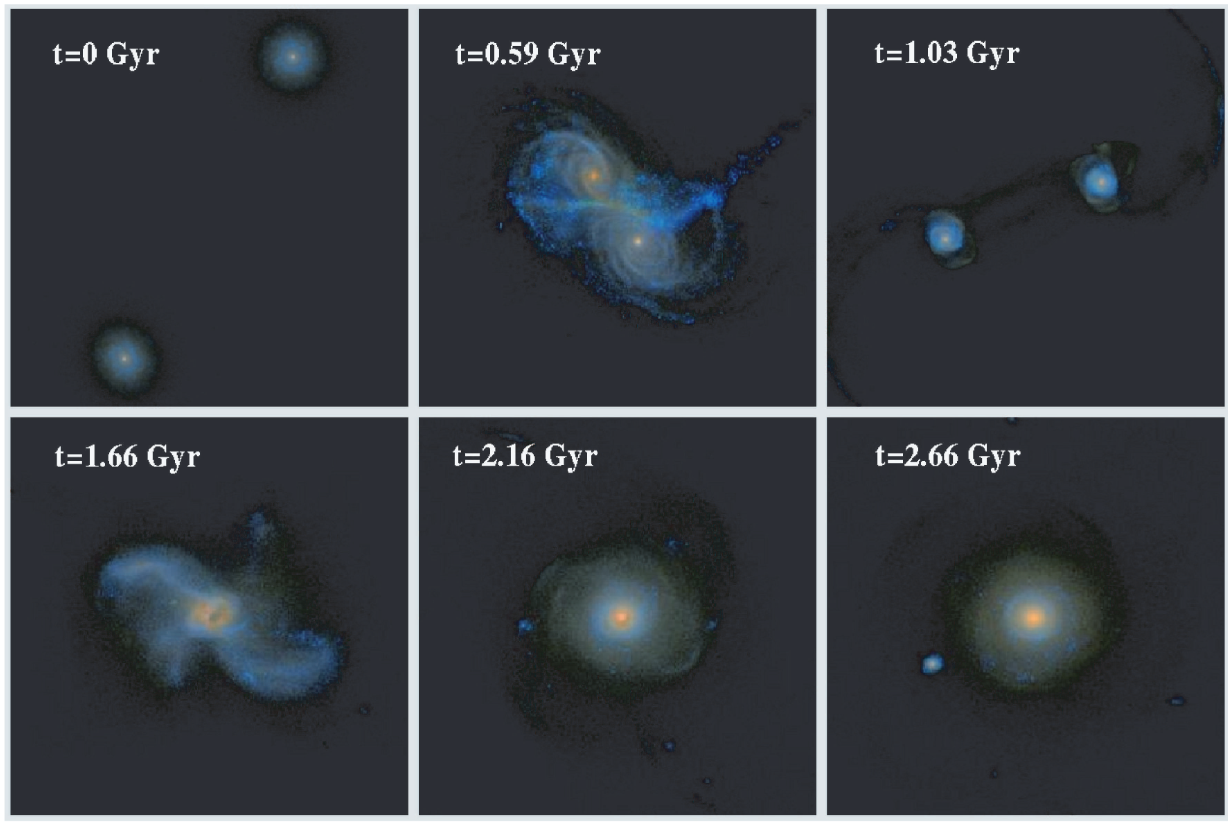
\includegraphics[width=\linewidth]{merger.png}
%     \caption{
%         A simulated merger of two Sbc galaxies from \cite{Lotz+2008}.
%         From right to left, the top row shows the two undisturbed pre-merger progenitors, the first pass, and the maximal separation after the first pass.
%         The bottom row shows the merger of the nuclei of the galaxies, the remnant 0.5 Gyr post-merger, and the remnant 1.0 Gyr post-merger.
%         }
%     \label{fig:merger}
% \end{figure}

% State why this topic matters to our understanding of galaxy evolution
Stepping back, a \textbf{galaxy} is defined as a gravitationally bound set of stars whose properties cannot be explained by a combination of baryons (gas, dust, and stars) and Newton's laws of gravity \citep{Willman+2012}, and thus \textbf{galaxy evolution} encompasses the change of galaxies over time and the formation of structures seen in galaxies today.
Studying the morphology of galaxy merger remnants is incredibly important for understanding galaxy evolution because most galaxies are affected by mergers and interactions \citep{Barnes+1992}.
For one, knowing how merger remnants look will aid us in identifying past merger events, helping us constrain merger rates and timescales throughout the history of the universe \citep{Lotz+2008}. 
Additionally, as stated before, the morphology of the remnant is heavily influenced by the properties of the parent galaxies and the collision, so knowing precisely how the remnant morphology changes with these factors can allow us to glean information about the progenitors \citep{Barnes+1992}.
In particular, we care about major merger events between spirals because they are thought to be a significant formation route for elliptical and spheroidal galaxies \citep{Barnes+1992}. 
However, there are other potential formation pathways for ellipticals and spheroids that must be accounted for \citep{Lotz+2008}.
Thus, studying the morphology of major merger remnants will help us to better distinguish between ellipticals and spheroids formed in different ways, allowing us to see the true prevalence of major mergers in elliptical galaxy formation and better understand the link between spirals and ellipticals.

% Overview of our current understanding of the topic in galaxy evolution
As it stands, we know a fair amount about how the properties of the progenitor spirals affect the morphology of the remnant.
For example, the kinematics of the collision and pre-merger progenitor orbits \citep{Barnes+1992, Duc2013}, as well as gravitational interactions of the dark matter halos of the progenitors \citep{Barnes+1992} are all important factors. 
% The kinematics of the merger are one important factor; a merger of two galaxies with high orbital angular momentum tends to produce oblate, rapidly rotating spheroids --- this is true in general in any case where the parent galaxies merge in a way that leaves the remnant with a high angular momentum --- whereas head-on collisions usually create prolate spheroids \citep{Barnes+1992}. 
% Similarly, prograde orbits pre-merger usually leave remnants with long, narrow tidal tails, as opposed to the shorter, more diffuse plumes associated with retrograde orbits \citep{Duc2013}. 
% The dark matter halos of the merging galaxies also play a vital role in the merger, as their interactions with each other actually cause the most angular momentum loss. 
% Generally, the progenitors' disks and bulges will also lose most of the their angular momentum to interacting with their own disturbed halos, only really interacting with the disk and bulge when they collide and merge; this is why remnants tend to still have dense, luminous central bulges \citep{Barnes+1992}.
In particular, though, dry galaxy major mergers tend to produce rounder, more elliptical remnants, whereas wet major mergers tend to produce more oblate, disk-like galaxies.
This occurs because as the gas acquires angular momentum during the merger, it tends to flatten out into a rotating disk at the center \citep{Eliche-Moral+2018}.
%On the other hand, large bulges tend to be more conducive to forming massive ellipticals \citep{Barnes+1992}.
Generally, it's thought that the vast majority of major mergers between spirals create ellipticals; however, simulations such as those by \cite{Eliche-Moral+2018} have shown that these mergers can create significant amounts of very oblate, disk-like remnants, even as far as S0 galaxies on the borderline between ellipticals and spirals, despite concerns that major mergers were too "catastrophic" to allow for an ordered disk to form, as shown in Fig. \ref{fig:morphs}.
\begin{figure}
    \centering
    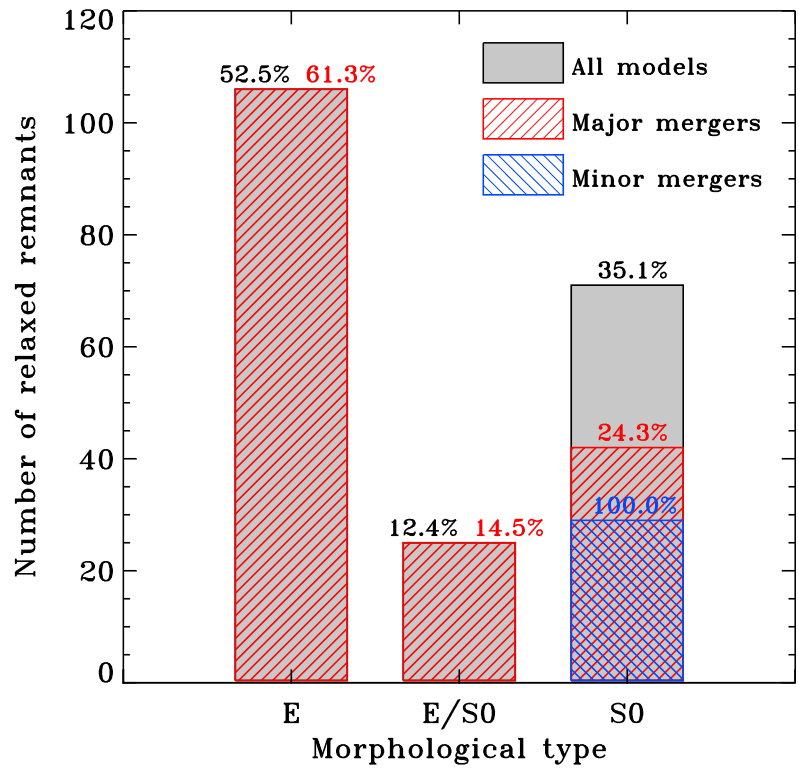
\includegraphics[width=0.8\linewidth]{morphs.png}
    \caption{
        Distribution of remnant morphological types across a sample of 202 merger simulations from \cite{Eliche-Moral+2018}.
        Percentages shown are calculated with respect to the total sample, as well as the samples of major mergers and minor mergers separately.
        Ellipticals dominate the major merger and overall sample, but S0 types are more prevalent than expected. 
        This indicates that major mergers may not be so "catastrophic" that it is is impossible for an ordered disk to form in the remnant.
        }
    \label{fig:morphs}
\end{figure}
    
% What are the open questions related to this topic?
There are still many questions left unanswered relating to major mergers and remnant morphology, though. 
For example, what is the precise relationship between bulges and ellipticals? 
What is the complete range of remnant dynamics and orbital structures that can be produced by a merger? \citep{Barnes+1992}
What are the exact roles played by mergers and and other evolutionary mechanisms in transforming spirals into elliptical, spheroidal and S0 galaxies? \citep{Eliche-Moral+2018}
Is more discrete formation through mergers preferred, or more continuous methods like cold gas accretion? \citep{Lotz+2008}
How does this change with redshift?
Questions like these are the ones that full simulations of mergers, careful analysis of the morphology of the remnants, and comparisons to real or suspected remnants will be able to answer, especially in the era of abundant JWST data of high redshift galaxies.

% This Project
\section{This Project}

In this paper, we will investigate the morphology of the stellar remnant of the Milky Way and M31 major merger.
More specifically, I will take advantage of the available simulation of this merger from \cite{van_der_Marel+2012} to describe the 3D structure of the remnant, rather than sticking to a 2D projection onto the sky.
I would perform this analysis on both the remnant galaxy as a whole, and at various radii within the remnant.

The main open question I will be addressing the role of mergers in transforming spiral galaxies into elliptical, spheroidal and S0 galaxies. 
Additionally, I will be contributing to answering the question of what the complete range of remnant orbital structures that can be produced by a merger is. 

The first question is important to answer because ellipticals being typically found in very dense clusters, being more compact in the past, and having little to no present star formation, indicating an environmentally cut off gas supply, suggests that mergers, in particular dry mergers of disk galaxies as described above, are important to their evolution. 
However, this does not rule out other evolutionary mechanisms, such as "inside-out" growth, in which a compact elliptical expands outwards over time as a result of minor mergers with smaller ellipticals.
Thus answering this question will help us untangle the dominant evolutionary mechanism for ellipticals (potentially at different redshifts).
In particular, my study will help identify morphological indicators of elliptical remnants of dry spiral mergers.
As for the second question, as stated above, knowing the complete range of orbital structures a merger can produce will help us identify merger remnants in general, as well as characterize the mergers that produced them and the overall frequency of galaxy mergers.
Again, my study will add to this knowledge base and enable better characterization and identification of dry major spiral merger remnants specifically.

% Methodology!!!
\section{Methodology}

For this study, I used the simulation of the Milky Way-M31 merger from \cite{van_der_Marel+2012}.
They ran collisionless $N$-body simulations of the MW-M31-M33 system (although M33 is not considered in this study, as it is not part of the merger), meaning each galaxy was represented by a collection of $N$ particles (with $N$ being some large number) which are allowed to interact with each other using Newton's law of gravity.
The initial conditions of M31 and the MW were chosen to be as close as possible to their present-day states. 
In particular, the orientations of the galaxies, the scale lengths of their disks and bulges, and the bulge masses were all based on literature values, and the center-of-mass positions and velocities and virial masses were chosen to agree with observational results.
Disks were modelled with exponential profiles, bulges with $R^{1/4}$ profiles, and dark matter halos with Hernquist profiles. 
It is to be noted that only dark matter and stellar mass was included, ignoring the gas because it comprises a small fraction of the mass and its removal allows for higher-resolution calculations.
The simulation data itself are comprised of snapshot files for each galaxy at specified time intervals over the course of the simulation that contain the velocities and positions of every particle in each galaxy.

I looked at a snapshot of the remnant 2 Gyr after the merger occured (Snap Number 595), so I can compare the result with the prediction that relaxed S0 remnants can form roughly 1 -- 2 Gyr after the merger occurs.
I used high-resolution snapshot files so that I can get as accurate a picture of the structure of the remnant as possible, and lower the resolution to whatever degree I needed if necessary.
The first step was to calculate the center of mass (CoM) of the remnant from the CoMs of the bulge and disk of the MW and M31. 
My next step was then to make the actual remnant "object" that I will analyze by making one position and one velocity array containing the bulge and disk particles of M31 and the MW and converting them to the remnant center of mass frame. 
I used these positions and velocities to rotate the remnant such that its angular momentum was aligned with the z-axis, allowing me to observe the remnant "edge-on" and "face-on."
The following steps, which are pictured in Fig. \ref{fig:methods}, I repeated for the projections of the remnant onto the xy, yz, and xz plane to get a full picture of the 3D structure of the remnant.
\begin{figure}[h!]
    \centering
    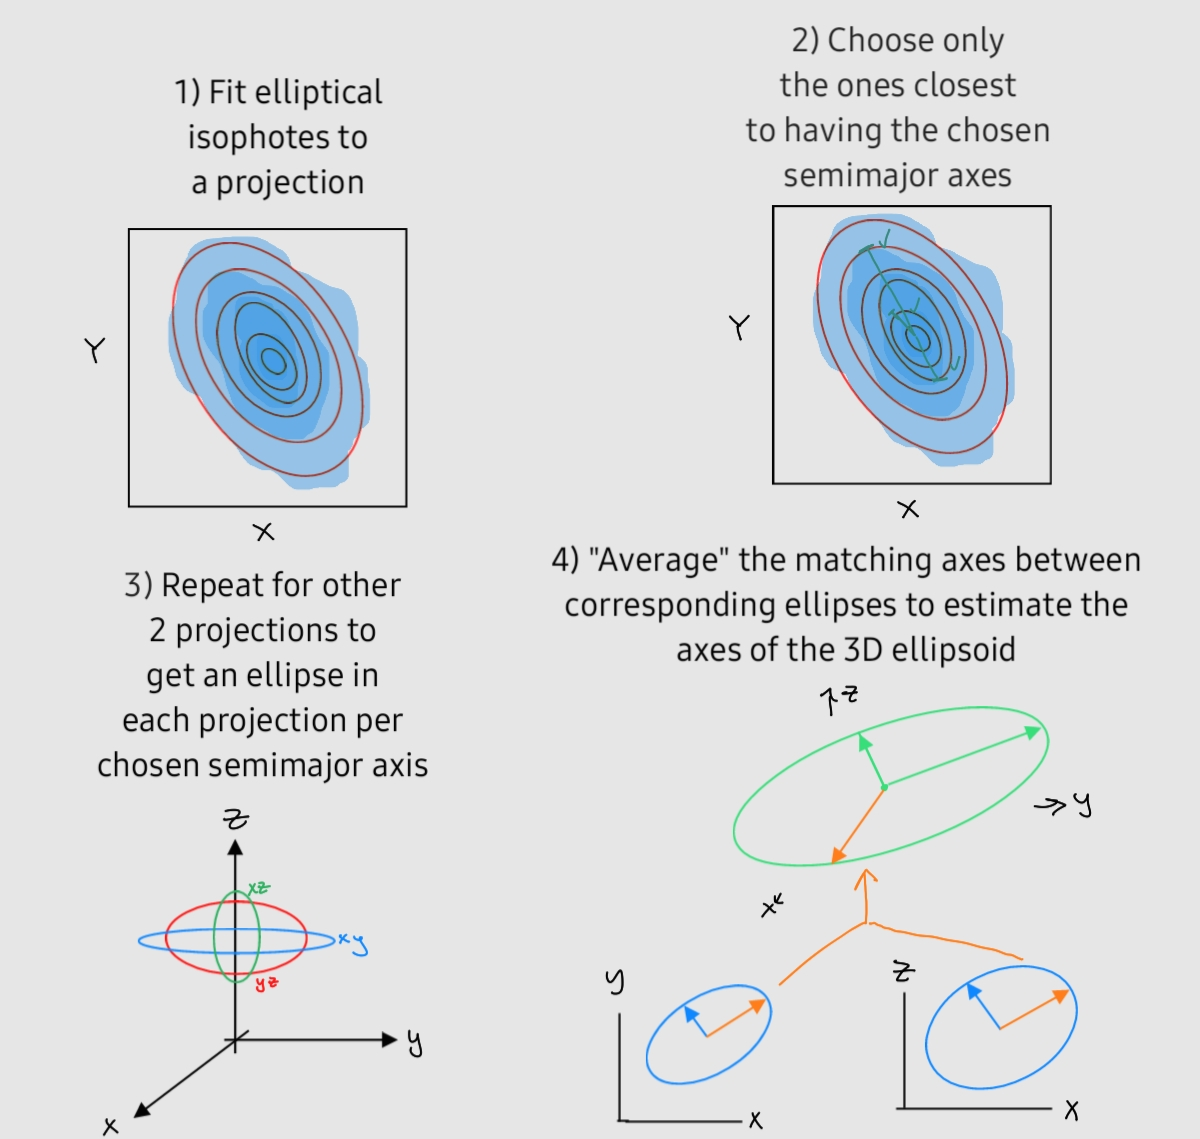
\includegraphics[width=0.8\linewidth]{methods.jpg}
    \caption{
        A visualization of the process of finding the 3D structure of the remnant at various "radii." You first fit 2D elliptical isophotes to the projections of the remnant using \texttt{photutils.isophote}, choose the ones with semimajor axes closest to the chosen "radii", then use the averaged like axes of the ellipses to estimate a 3D ellipsoid fit at each "radius."
    }
    \label{fig:methods}
\end{figure}
% Using \texttt{density\_contour()} from Lab 7, I then fitted 10 isodensity contours to these particles, with the first containing 10\% of the total particles and the last 100\%.
% From there, I fitted an ellipse to each of the contours using least squares fitting, and extracting its semimajor axis $a$ and semiminor axis $b$, as well as the other geometrical properties, like the tilt angle $\theta$ and the center position $(x_o, y_o)$.
Using \texttt{photutils.isophote}, I fitted a series of elliptical isophotes (i.e. contours of regions with the same "brightess," which in this case is really particle density) to each projection of the remnant.
I then chose a range of semimajor axis lengths that covered the remnant, and found the ellipses that fit them most closely in each projection.
For large semimajor axes, often photutils did not fit ellipses large enough, so it would match the same ellipse to multiple semimajor axes; I thus manually selected only for ellipses below a certain radius depending on where these repeats began.
For these ellipses, I then extracted their semimajor and semiminor axes and determined which of the coordinate axes they aligned with best, sorting them accordingly.
I then approximated 3D ellipsoid fits by taking elliptical isophotes fit to the same semimajor axis in each of the three projections, and treating their axes as 2D vector projections of the 3D axes of the ellipsoid.
This allowed me to determine as 3D vectors the ellipsoid axes by averaging the common nonzero component of the relevant 2D ellipse axes and taking the sums of their other two.
Doing this for all 3 axes for every set of 3 elliptical isophotes gave me the ellipsoid fits as a function of "radius."
From here, I used the lengths of the 3 axes of each ellipsoid to classify the remnant's morphology at each "radius."

To find the CoM position $R_r$ and velocity $V_r$ of the remnant, I used the typical center of mass equations:
\begin{equation} \label{eq:comR}
    R_r = \frac{\sum_{galaxies}\sum_{components}M_iR_i}{\sum_{galaxies}\sum_{components}M_i}
\end{equation}
\begin{equation} \label{eq:comV}
    V_r = \frac{\sum_{galaxies}\sum_{components}M_iV_i}{\sum_{galaxies}\sum_{components}M_i}
\end{equation}
where $M_i$ is the mass of a galaxy component, $R_i$ is its CoM position, and $V_i$ is its CoM velocity, and we are summing over the bulges and disks of M31 and the MW.
% The main calculation in my code, though, was finding the geometrical parameters $a$, $b$, $x_o$, $y_o$, and $\theta$ of the fitted ellipses.
% The actual equation of an ellipse used for the least squares fit is 
% \begin{equation}\label{eq:lstsqfit}
%     \alpha x^2 + \beta xy + \gamma y^2 + \eta x + \kappa y + \mu = 0
% \end{equation}
% whereas the equation of an ellipse expressed geometrically (with the quantities we want) is 
% \begin{equation}\label{eq:geom}
%     \frac{(X\cos\theta+Y\sin\theta)^2}{a^2} + \frac{(X\sin\theta+Y\cos\theta)^2}{b^2} = 1 
% \end{equation}
% where $X=x-x_o$ and $Y=y-y_o$.
% Solving equations \ref{eq:lstsqfit} and \ref{eq:geom} then yields the following relations for the geometrical properties:
% \begin{equation}\label{eq:a}
%     a = - \frac{\sqrt{2(\alpha\kappa^2+\gamma\eta^2 - \beta\eta\kappa + (\beta^2 - 4\alpha\gamma)\mu)(\alpha+\gamma + \sqrt{(\alpha-\gamma)^2+\beta^2}}}{\beta^2-4\alpha\gamma}
% \end{equation}
% \begin{equation}\label{eq:b}
%     b = -\frac{\sqrt{2(\alpha\kappa^2+\gamma\eta^2 - \beta\eta\kappa + (\beta^2 - 4\alpha\gamma)\mu)(\alpha+\gamma - \sqrt{(\alpha-\gamma)^2+\beta^2}}}{\beta^2-4\alpha\gamma}
% \end{equation}
% \begin{equation}\label{eq:xo}
%     x_o = \frac{2\gamma\eta - \beta\kappa}{\beta^2 - 4\alpha\gamma}
% \end{equation}
% \begin{equation}\label{eq:yo}
%     y_o = \frac{2\alpha\kappa - \beta\eta}{\beta^2 - 4\alpha\gamma}
% \end{equation}
% \begin{equation}\label{eq:theta}
%     \theta = \frac{1}{2}\arctan2(-\beta,\gamma-\alpha)
% \end{equation}
% with arctan2 being the 2-argument arctangent function. (I will figure out how to make those equations not overflow the page, I promise).
% From there, once I have the elliptical fits for a specific density contour in all three projections, I will estimate the 3D axis $A$ (the closest to the $z$-axis) as the average of the closest axis to the $z$ in the xz and yz projections, and similarly for $B$ (the closest to the $y$ axis) and $C$ (the closest to the $z$ axis).
The most major calculation I did, however, was determining the 3D axes of the ellipsoid fits.
As an example, say I am finding the ellipsoid axis closest to the $y$-axis, $R_y$.
I would then take the two corresponding 2D elliptical isophotes --- the ones in the $xy$ and $yz$ projections --- and find their axes closest to $y$, $r_{xy}$ and $r_{yz}$, and their position angles $\alpha_{xy}$ and $\alpha_{yz}$.
Represented as 3D vectors, we see that
\begin{equation}
\begin{split}  
    & \vec{r}_{xy} = (r_{xy}\cos\alpha_{xy} \ , \ r_{xy}\sin\alpha_{xy} \ , \ 0) 
    \\ 
    & \vec{r}_{yz} = (0 \ , \ r_{yz}\cos\alpha_{yz} \ , \ r_{yz}\sin\alpha_{yz}) \ \ .
\end{split}
\end{equation}
Then I estimated $\vec{R}_y$ as
\begin{equation}
\begin{split}
    \vec{R}_y = (&r_{xy}\cos\alpha_{xy} \ , 
    \\ &  [r_{xy}\sin\alpha_{xy} + r_{yz}\cos\alpha_{yz}]/2 \ ,
    \\ & r_{yz}\sin\alpha_{yz}\textbf{}) \ \ ,
\end{split}
\end{equation}
meaning we simply had that $R_y = |\vec{R}_y|$.
The process for the 3D axes closest to the $x$ and $z$-axes was similar.
Once I had the axes for a given ellipsoid, I ordered them by length and let $A$ be the largest, $C$ the smallest, and $B$ the median.
Finally, I computed the axis ratios $q_1 = B/A$ and $q_2 = C/A$ and then used them to determine the triaxiality parameter $T$ for the ellipsoid as defined in \cite{Quenneville+2022}:
\begin{equation} \label{eq:triax}
    T = \frac{1-q_1^2}{1-q_2^2} \ \ .
\end{equation}
If $T=0$, the ellipsoid is \textbf{oblate} ($A=B>C$, "squashed"), if $T=1$, it's \textbf{prolate} ($A>B=C$, "stretched"), and if $0<T<1$, it's \textbf{triaxial} (all its axes are different lengths).

\begin{figure*}
    \centering
    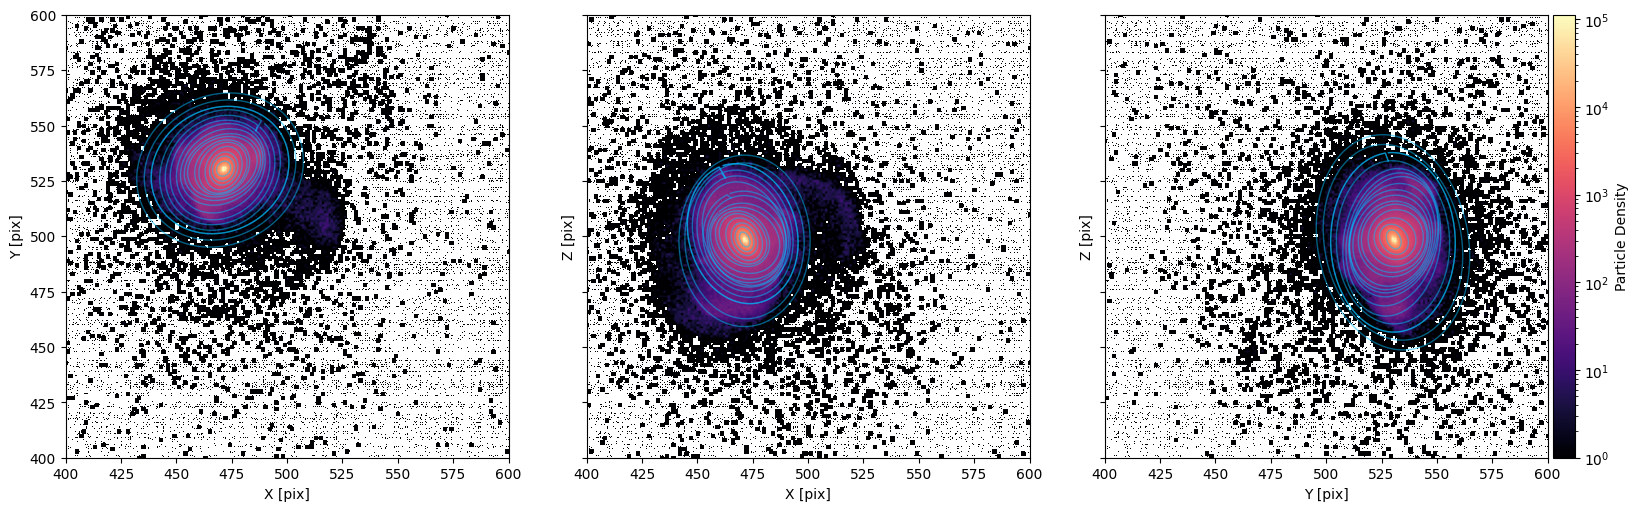
\includegraphics[width=0.85\linewidth]{ellipse_fits.png}
    \caption{Zoomed in 2D histograms of the projections of the MW-M31 remnant in the XY, XZ, and YZ planes. The colors correspond to the density of particles in logarithmic scale as shown on the colorbar to the right, with lighter colors meaning a higher density. Overplotted in blue are the elliptical isophotes fitted by \texttt{photutils.isophote} that I used for the ellipsoid fits. Overall, in each projection, the remnant appears to become more elliptical further from the center. The XZ and YZ projections also generally have more elongated isophotes than the XY projection. Already the remnant is shown to most likely be triaxial.}
    \label{fig:ell_fits}
\end{figure*}

One plot I will make will be of the fitted elliptical isophotes that I used for the ellipsoid fits overplotted on each projection of the remnant for both snapshots; this will help both visually verify how accurate the fitted ellipses are and show visually how the remnant shape and inclination changes with radius. 
I will quantify the change in 3D shape similarly by plotting $q_1$, $q_2$, and $T$ versus the largest axis of the fitted ellipsoids, $A$.
These plots will show not only the shape of the remnant, but whether it has any significant substructure.

My hypothesis is that the remnant will be spheroidal, or maybe slightly oblate, but certainly not as oblate or disk-like as an S0 galaxy. 
M31 and the Milky Way are both rather gas-poor galaxies residing in the "Green Valley," so I do not expect them to have enough gas to allow the disk to reform post-merger, even in the much later of the two snapshots.


\section{Results}

I first plotted 2D histograms of the projections of the remnant onto each of the three coordinate planes with the fitted isophotes overlaid in order to visually inspect them (Figure \ref{fig:ell_fits}). 
The colors of the underlying histogram correspond to the density of stellar particles in logarithmic scale, with lighter colors meaning higher densities.
We can clearly see that in the center of the remnant, the fitted isophotes appear more circular, and gradually become more elliptical as they increase in semimajor axis. 
Additionally, the projections including the z-axis seem to have more elongated isophotes overall than the projection into the XY plane, especially in the YZ plane.
This already shows us that the remnant will likely be triaxial for the most part.

\begin{figure}
    \centering
    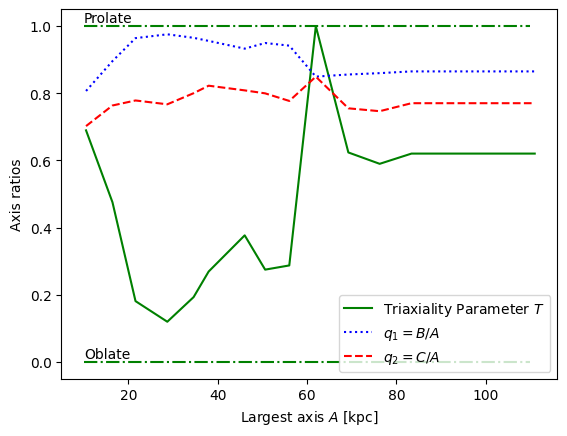
\includegraphics[width=0.85\linewidth]{axis_ratios.png}
    \caption{Plot of the two axis ratios $q_1$ (blue dotted line) and $q_2$ (red dashed line) as well as the triaxiality parameter $T$ (solid green line) as a function of the length of the largest axis $A$ for each of the 3D ellipsoid fits. The horizontal green dotted-dashed lines indicate the limits of $T$ corresponding to a prolate or oblate ellipsoid. The remnant is mostly  triaxial although between about 20 -- 60 kpc it is surprisingly close to oblate, which is likely most representative of the actual remnant morphology.}
    \label{fig:axis_ratios}
\end{figure}
To quantitatively show this, however, I plotted the axis ratios $q_1 = B/A$ and $q_2 = C/A$, as well as the triaxiality parameter $T$ (Equation \ref{eq:triax}) for each 3D fit from the isophotes as a function of the length of the largest axis (Figure \ref{fig:axis_ratios}). 
I also plotted the limits of $T$ that would indicate a prolate or oblate ellipsoid.
Here we can see more clearly that overall, $T$ lies fairly solidly in between 0 and 1 for the most part, indicating a triaxial shape.
Surprisingly, between about 20 -- 60 kpc from the center, the remnant seems to be more oblate than prolate, although still clearly triaxial.


\section{Discussion}

The shape of the remnant for all radii is clearly triaxial, as the triaxiality parameter $T$ stays solidly between 0 and 1.
The one exception is at roughly 65 kpc, although given the suddenness and isolation of this spike to being prolate, and the relatively low density of particles at this point, it's rather dubious.
However, between 20 -- 60 kpc, its shape tends to be more oblate, surprisingly, with $0.1 < T < 0.4$ roughly. 
While the triaxial, tending slightly towards prolate outermost shape of the remnant would be more in line with my prediction of a spheroidal or prolate remnant, the 20 -- 60 kpc range is arguably most reflective of its actual shape, given the very low density of particles in the outer parts of the galaxy.
So the remnant is most likely closer to oblate, which directly contradicts my expectation that it would \textit{not} be oblate.

This triaxial, slightly oblate shape of the remnant does not agree with much existing work in the literature. 
For one, this is a dry merger that produced an oblate-ish remnant despite the lack of gas to flatten into the disk as \cite{Barnes+1992} expected. 
This could then indicate that the oblate-ish shape was preserved or reformed in just the stellar matter from the progenitor galaxies, the Milky Way and M31. 
This could actually support the claim made by \cite{Eliche-Moral+2018} that major mergers are not too "violent" to leave a disk-like remnant; while this remnant is not disk-like enough to be an S0 galaxy, it still shows that oblate-ish remnants are not out of the realm of possibility.
This result thus shows that dry major mergers can be important formation mechanism of a more diverse range of elliptical galaxies than just the traditional round ellipticals and spheroidals. 
This could imply that broadly ellipticals as a whole are even more commonly formed from mergers than originally thought.
Additionally, adding to our lexicon of possible merger remnant morphologies not only allows us to more frequently and accurately identify merger remnants, but also the types of mergers that created them.

There are a few uncertainties in the analysis that are worth noting, however. 
A notable one is the fitting of the elliptical isophotes.
\texttt{photutils.isophote} fits the isophotes wherever they seem most convenient, and then can return to you the one closest to having a given semimajor axis; as such it is possible that the elliptical isophotes I used to construct the 3D ellipsoids may not actually "match," i.e. trace the same part of the remnant. 
Another concern is the fitting of the outer isophotes, as the outer edge of the remnant has a short tidal tail that likely skewed the fits.
The other larger source of uncertainty stems from my method of averaging the vectorized forms of the common axes of the elliptical fits on each projection to estimate a 3D ellipsoid fit. 
This method unfortunately does not account for differences in the centers of the isophotes, as well as whether the averaged 3D axes would be perfectly perpendicular to each other.
This is only compounded by the aforementioned issues with the 2D isophotes.
However, if 2D isophotes are chosen correctly, the geometry of the galaxy itself would theoretically not allow this to be too much of an issue.


%% Conclusion
\section{Conclusion}

Morphology, or shape, is a particularly useful way of characterizing the remnants of dry major mergers of spiral galaxies, i.e. collisions between gas-poor spiral galaxies of approximately the same mass.
Studying remnant morphology allows us to identify merger remnants and thus constrain merger rates and their importance in the formation of galaxies, especially elliptical galaxies.
To further investigate this topic, I used the collisionless $N$-body simulation of the Milky Way-M31 merger by \cite{van_der_Marel+2012}, where initial conditions of the two galaxies were set as close as possible to their present states and their particles were then allowed to interact via Newton's law of gravity.
In particular, I studied the three-dimensional morphology of the remnant as a function of radius. 

I found that while the remnant is very solidly triaxial throughout, with the triaxiality parameter $T$ never reaching 0 or 1, for "radii" between 20 and 60 kpc its shape tends towards \textit{oblate}.
Further out, the densities of particles are incredibly low, meaning that this more representative of the overall remnant morphology.
However, this finding disagrees with my hypothesis, as it was generally expected that gas-poor major mergers of spirals are too "destructive" to allow disk-like, oblate structures to form.
By showing that more oblate-ish remnants \textit{can} form from such mergers, this could mean that mergers play a significant role in forming a broader range of ellipticals than just spheroidal and prolate elliptical galaxies. 
In fact, it could indicate that mergers could be a more common formation mechanism for ellipticals in general.

In the future, I would like to improve my code by ensuring that I am using 2D isophotes that trace the same portion of the galaxy in each plane. 
One way of doing this would be the method I had originally intended on using, i.e. fitting an ellipse using least-squares fitting to isodensity contours on the galaxy. 
This would also give me much more control over the "radius" at which I'm fitting an ellipse.
However, although it was not feasible for the scope of this project, the best improvement I could make to my methodology is to directly fit ellipsoids to the 3D remnant particle positions.
Turning to the simulation, as previously mentioned, the gas in the M31 and the Milky Way was left out of the simulations to ensure faster, higher-resolution simulations could be completed, since neither galaxy contains much gas.
However, given the important role gas plays in the formation of a disk, it may be useful to include gas in the simulations to see if it affects how oblate the final remnant is.
Looking forward, though, I would like to investigate the change in the remnant's morphology over time.
This would constrain relaxation timescales for remnants and the extent to which remnant morphologies change after a merger.


%% Acknowledgements
\section{Acknowledgements}
I would like to thank Hayden Foote for the coding advice he gave during the in-class hack days, Himansh Rathore for providing an example of ellipse fitting with \texttt{photutils.isophote}, and Dr. Gurtina Besla for general advice for the project.
I would also like to thank my friend Ellen Jesina and my partner Alex for their emotional support throughout this process.
This work made use of the following software packages: \texttt{astropy} \citep{astropy:2013, astropy:2018, astropy:2022}, \texttt{Jupyter} \citep{2007CSE.....9c..21P, kluyver2016jupyter}, \texttt{matplotlib} \citep{Hunter:2007}, \texttt{numpy} \citep{numpy}, \texttt{ipython} \citep{ipython}, and \texttt{python} \citep{python}.
This research made use of Photutils, an Astropy package for detection and photometry of astronomical sources \citep{Photutils_8248020}.
Software citation information aggregated using \texttt{\href{https://www.tomwagg.com/software-citation-station/}{The Software Citation Station}} \citep{software-citation-station-paper, software-citation-station-zenodo}.
We respectfully acknowledge the University of Arizona is on the land and territories of Indigenous peoples. Today, Arizona is home to 22 federally recognized tribes, with Tucson being
home to the O’odham and the Yaqui. The University strives to build sustainable relationships with sovereign Native Nations and Indigenous communities through education offerings,
partnerships, and community service.


%% Bibliography!

\bibliography{biblio}{}
\bibliographystyle{aasjournal}


\end{document}

